\chapter{Collection of Results} \label{chp:totalresults}

\section{Energy distribution} \label{sec:energydistribution}
In this appendix, we present the energy distribution between kinetic energy, external potential energy and interaction energy for single quantum dots containing up to 20 particles in two and three dimensions. These results are interesting for the validation of the virial theorem, described in section \ref{sec:virial}, but they also makes it possible to compare how the energy spread in two  and three dimensions for an equal number of particles 

\subsection{Two dimensions}
\begin{table}[H]
	\caption{This table shows how the total energy ($\langle\hat{H}\rangle$) is distributed between kinetic energy ($\langle\hat{T}\rangle$), external potential energy ($\langle\hat{V}_{\text{ext}}\rangle$) and interaction energy ($\langle\hat{V}_{\text{int}}\rangle$) of two-dimensional circular quantum dots at a wide range of frequencies $\omega$. A standard variational Monte-Carlo wave function is used. The energy is given in units of $\hbar$, and the numbers in parenthesis are the statistical uncertainties in the last digit.}
	\label{tab:splitfrequencyQDVMC}
	\begin{tabularx}{\textwidth}{R{1cm}rrcR{2.3cm}R{2.3cm}R{2.3cm}R{2.3cm}R{1cm}} \hline\hline
		&\makecell{\\ \phantom{$N$} \\ \phantom{=}} & $\omega$ && \multicolumn{1}{c}{$\langle \hat{H}\rangle$} & \multicolumn{1}{c}{$\langle \hat{T}\rangle$} & \multicolumn{1}{c}{$\langle \hat{V}_{\text{ext}} \rangle$} & \multicolumn{1}{c}{$\langle \hat{V}_{\text{int}} \rangle$} & \\ \hline \\
		&2 & 0.01 && 0.074070(8) & 0.00947(3) & 0.02732(5) & 0.03728(4) \\
		&& 0.1 && 0.44129(1) & 0.09117(9) & 0.1789(1) & 0.17119(9) \\
		&& 0.28 && 1.02192(1) & 0.2477(1) & 0.4256(2) & 0.3487(1) \\
		&& 0.5 && 1.65974(1) & 0.4346(2) & 0.7057(2) & 0.5195(2)\\
		&& 1.0 && 2.99936(1) & 0.8523(3) & 1.3149(3) & 0.8321(2)\\
		&& 2.0 && 5.497567(8) & 2.0574(3) & 1.9931(3) & 1.4471(3) \\
		&& 3.0 && 7.881906(9) & 2.5028(5) & 3.6911(6) & 1.6880(3) \\ 
		&& 5.0 && 12.504211(8) & 5.1819(6) & 4.7651(6) & 2.5572(5) \\
		&& 10.0 && 23.65035(1) & 9.529(1) & 10.538(1) & 3.583(1) \\
		\hdashline \\
		
		&6 & 0.01 && 0.6982(1) & 0.02735(7) & 0.2427(3) & 0.4281(3) \\
		&& 0.1 && 3.5695(1) & 0.3201(3) & 1.2934(6) & 1.9560(5) \\
		&& 0.28 && 7.6219(1) & 0.9105(4) & 2.8821(9) & 3.8292(7) \\
		&& 0.5 && 11.8104(2) & 1.6710(7) & 4.535(1) & 5.6045(9)\\
		&& 1.0 && 20.1918(2) & 3.405(1) & 8.046(1) & 8.741(1)\\
		&& 2.0 && - & - & - & -\\
		&& 3.0 && 51.072(6) & 8.71(3) & 28.24(4) & 14.11(1) \\ 
		&& 5.0 && - & - & - & -\\
		&& 10.0 && - & - & - & -\\
		\hdashline \\
		
		&12 & 0.01 && 2.4972(3) & 0.05506(2) & 0.858(1) & 1.584(1)\\
		&& 0.1 && 12.3196(3) & 0.6885(6) & 4.393(2) & 7.238(2) \\
		&& 0.28 && 25.7049(4) & 2.090(1) & 9.355(2) & 14.260(2) \\
		&& 0.5 && 39.2421(5) & 3.939(2) & 14.564(3) & 20.739(3) \\
		&& 1.0 && 65.7928(5) & 8.536(3) & 24.874(4) & 32.383(3) \\
		&& 2.0 && 111.86(4) & 20.22(2) & 40.04(2) & 51.605(9) \\
		&& 3.0 && 155.5235(1) & 23(1) & 63(1) & 68.4(2) \\ 
		&& 5.0 && - & - & - & -\\
		&& 10.0 && - & - & - & -\\
		\hdashline \\
		
		&20 & 0.01 && 6.2097(8) & 0.1005(4) & 2.270(3) & 3.839(3) \\
		&& 0.1 && 30.086(1) & 1.243(1) & 10.587(4) & 18.257(4) \\
		&& 0.28 && 62.0755(7) & 3.902(2) & 22.228(5) & 35.946(4) \\
		&& 0.5 && 94.0433(9) & 7.823(3) & 33.938(6) & 52.282(5) \\
		&& 1.0 && 156.102(1) & 16.86(1) & 58.14(1) & 81.098(6) \\
		&& 2.0 && 262.0(4) & 39.3(4) & 93.57(7) & 129.05(4) \\
		&& 3.0 && 357.1(3) & 6(15) & 194(15) & 156.751(9) \\ 
		&& 5.0 && - & - & - & -\\
		&& 10.0 && - & - & - & -\\
		\hline \hline
	\end{tabularx}
\end{table} 

\begin{table}[H]
	\caption{This table shows how the total energy ($\langle\hat{H}\rangle$) is distributed between kinetic energy ($\langle\hat{T}\rangle$), external potential energy ($\langle\hat{V}_{\text{ext}}\rangle$) and interaction energy ($\langle\hat{V}_{\text{int}}\rangle$) of two-dimensional circular quantum dots at a wide range of frequencies $\omega$. A plain restricted Boltzmann machine wave function is used. The energy is given in units of $\hbar$, and the numbers in parenthesis are the statistical uncertainties in the last digit.}
	\label{tab:splitfrequencyQDRBM}
	\begin{tabularx}{\textwidth}{R{1cm}rrcR{2.3cm}R{2.3cm}R{2.3cm}R{2.3cm}R{1cm}} \hline\hline
		&\makecell{\\ \phantom{$N$} \\ \phantom{=}} & $\omega$ && \multicolumn{1}{c}{$\langle \hat{H}\rangle$} & \multicolumn{1}{c}{$\langle \hat{T}\rangle$} & \multicolumn{1}{c}{$\langle \hat{V}_{\text{ext}} \rangle$} & \multicolumn{1}{c}{$\langle \hat{V}_{\text{int}} \rangle$} & \\ \hline \\
		&2 & 0.01 && 0.07954(7) & 0.00872(2) & 0.03402(9) & 0.0368(1) \\
		&& 0.1 && 0.4743(1) & 0.08102(8) & 0.2082(2) & 0.1851(2) \\
		&& 0.28 && 1.0707(2) & 0.2047(1) & 0.4678(3) & 0.3983(3) \\
		&& 0.5 && 1.7234(2) & 0.3739(2) & 0.7611(3) & 0.5884(3)\\
		&& 1.0 && 3.0829(2) & 0.7691(2) & 1.3926(4) & 0.9212(3)\\
		&& 2.0 && 5.5936(3) & 1.6377(4) & 2.5507(5) & 1.4051(4) \\
		&& 3.0 && 7.9968(4) & 2.2346(5) & 4.0201(7) & 1.7422(4) \\ 
		&& 5.0 && 12.6070(4) & 3.8768(7) & 6.4292(9) & 2.3010(4) \\
		&& 10.0 && 23.6589(5) & 5.054(2) & 15.592(2) & 3.0129(6) \\
		\hdashline \\
		
		&6 & 0.01 && 0.7072(5) & 0.033(2) & 0.2660(4) & 0.4080(6) \\
		&& 0.1 && 3.7337(5) & 0.3251(3) & 1.4070(9) & 2.002(1) \\
		&& 0.28 && 7.9273(9) & 0.8684(6) & 3.009(1) & 4.050(2) \\
		&& 0.5 && 12.241(1) & 1.611(1) & 4.709(2) & 5.921(2)\\
		&& 1.0 && 20.716(1) & 3.391(1) & 7.914(3) & 9.411(2)\\
		&& 2.0 && - & - & - & -\\
		&& 3.0 && 49.415(1) & 10.309(3) & 21.456(4) & 17.649(2) \\ 
		&& 5.0 && - & - & - & -\\
		&& 10.0 && - & - & - & -\\
		\hdashline \\
		
		&12 & 0.01 && 2.5106(8) & 0.0682(2) & 0.893(1) & 1.549(1) \\
		&& 0.1 && - & - & - & - \\
		&& 0.28 && - & - & - & - \\
		&& 0.5 && 40.442(3) & 4.116(2) & 14.868(4) & 21.458(4) \\
		&& 1.0 && 67.614(3) & 8.953(3) & 25.207(6) & 33.455(5) \\
		&& 2.0 && - & - & - & -\\
		&& 3.0 && TIME & - & - & - \\ 
		&& 5.0 && - & - & - & -\\
		&& 10.0 && - & - & - & -\\
		\hdashline \\
		
		&20 & 0.01 && 6.217(2) & 0.1236(4) & 2.244(2) & 3.849(2) \\
		&& 0.1 && EXPL & - & - & - \\
		&& 0.28 && TIME & - & - & - \\
		&& 0.5 && 96.491(4) & 8.144(3) & 34.953(8) & 53.394(8) \\
		&& 1.0 && 159.645(5) & 17.12(5) & 58.74(5) & 83.397(9) \\
		&& 2.0 && - & - & - & -\\
		&& 3.0 && 362.52(1) & 57.005(9) & 148.08(2) & 157.43(1) \\ 
		&& 5.0 && - & - & - & -\\
		&& 10.0 && - & - & - & -\\
		\hline \hline
	\end{tabularx}
\end{table} 

\begin{table}[H]
	\caption{This table shows how the total energy ($\langle\hat{H}\rangle$) is distributed between kinetic energy ($\langle\hat{T}\rangle$), external potential energy ($\langle\hat{V}_{\text{ext}}\rangle$) and interaction energy ($\langle\hat{V}_{\text{int}}\rangle$) of two-dimensional circular quantum dots at a wide range of frequencies $\omega$. A restricted Boltzmann machine wave function with a simple Jastrow factor is used. The energy is given in units of $\hbar$, and the numbers in parenthesis are the statistical uncertainties in the last digit.}
	\label{tab:splitfrequencyQDRBMSJ}
	\begin{tabularx}{\textwidth}{R{1cm}rrcR{2.3cm}R{2.3cm}R{2.3cm}R{2.3cm}R{1cm}} \hline\hline
		&\makecell{\\ \phantom{$N$} \\ \phantom{=}} & $\omega$ && \multicolumn{1}{c}{$\langle \hat{H}\rangle$} & \multicolumn{1}{c}{$\langle \hat{T}\rangle$} & \multicolumn{1}{c}{$\langle \hat{V}_{\text{ext}} \rangle$} & \multicolumn{1}{c}{$\langle \hat{V}_{\text{int}} \rangle$} & \\ \hline \\
		&2 & 0.01 && 0.075267(3) & 0.00738(2) & 0.03071(8) & 0.03718(8) \\
		&& 0.1 && 0.44858(6) & 0.07539(8) & 0.1990(2) & 0.1742(1) \\
		&& 0.28 && 1.03470(7) & 0.2163(1) & 0.4547(2) & 0.3637(2) \\
		&& 0.5 && 1.67739(9) & 0.3913(2) & 0.7450(3) & 0.5411(2)\\
		&& 1.0 && 3.0259(1) & 0.7857(3) & 1.3958(4) & 0.8444(3)\\
		&& 2.0 && 5.5254(1) & 1.6572(3) & 2.5447(5) & 1.3234(3) \\
		&& 3.0 && 7.9409(1) & 2.2162(5) & 4.0834(7) & 1.6413(3) \\ 
		&& 5.0 && - & - & - & -\\
		&& 10.0 && - & - & - & -\\
		\hdashline \\
		
		&6 & 0.01 && 0.7006(3) & 0.0376(2) & 0.2467(4) & 0.4163(4) \\
		&& 0.1 && 3.6458(4) & 0.2376(3) & 1.3652(9) & 2.043(1) \\
		&& 0.28 && 7.7347(4) & 0.7603(4) & 3.000(1) & 3.974(1) \\
		&& 0.5 && 11.9392(5) & 1.4801(5) & 4.678(1) & 5.781(1) \\
		&& 1.0 && - & - & - & - \\
		&& 2.0 && - & - & - & -\\
		&& 3.0 && - & - & - & - \\ 
		&& 5.0 && - & - & - & -\\
		&& 10.0 && - & - & - & -\\
		\hdashline \\
		
		&12 & 0.01 && 2.4950(5) & 0.07(2) & 0.845(4) & 1.58(2) \\
		&& 0.1 && 13.11(6) & 0.29(5) & 4.8(1) & 8.1(2) \\
		&& 0.28 && 26.340(2) & 1.917(2) & 10.006(4) & 14.417(4) \\
		&& 0.5 && 41.28(1) & 4.07(1) & 16.948(5) & 20.265(4) \\
		&& 1.0 && 70.0(2) & 7.7(2) & 33.615(9) & 28.723(4) \\
		&& 2.0 && - & - & - & -\\
		&& 3.0 && - & - & - & - \\ 
		&& 5.0 && - & - & - & -\\
		&& 10.0 && - & - & - & -\\
		\hdashline \\
		
		&20 & 0.01 && 6.239(2) & 0.1372(6) & 2.184(2) & 3.919(3) \\
		&& 0.1 && 30.624(3) & 1.487(2) & 10.893(5) & 18.243(5) \\
		&& 0.28 && 62.786(3) & 3.190(2) & 22.782(7) & 36.814(6) \\
		&& 0.5 && 94.755(3) & 6.709(2) & 34.845(7) & 53.200(6) \\
		&& 1.0 && 156.816(4) & 15.340(3) & 59.931(9) & 81.545(7) \\
		&& 2.0 && - & - & - & -\\
		&& 3.0 && 358.71(4) & 51.02(4) & 153.52(2) & 154.16(1) \\ 
		&& 5.0 && - & - & - & -\\
		&& 10.0 && - & - & - & -\\
		\hline\hline
	\end{tabularx}
\end{table}

\begin{table}[H]
	\caption{This table shows how the total energy ($\langle\hat{H}\rangle$) is distributed between kinetic energy ($\langle\hat{T}\rangle$), external potential energy ($\langle\hat{V}_{\text{ext}}\rangle$) and interaction energy ($\langle\hat{V}_{\text{int}}\rangle$) of two-dimensional circular quantum dots at a wide range of frequencies $\omega$. A restricted Boltzmann machine with Padé-Jastrow wave function is used. The energy is given in units of $\hbar$, and the numbers in parenthesis are the statistical uncertainties in the last digit.}
	\label{tab:splitfrequencyQDRBMPJ}
	\begin{tabularx}{\textwidth}{R{1cm}rrcR{2.3cm}R{2.3cm}R{2.3cm}R{2.3cm}R{1cm}} \hline\hline
		&\makecell{\\ \phantom{$N$} \\ \phantom{=}} & $\omega$ && \multicolumn{1}{c}{$\langle \hat{H}\rangle$} & \multicolumn{1}{c}{$\langle \hat{T}\rangle$} & \multicolumn{1}{c}{$\langle \hat{V}_{\text{ext}} \rangle$} & \multicolumn{1}{c}{$\langle \hat{V}_{\text{int}} \rangle$} & \\ \hline \\
		&2 & 0.01 && 0.074107(8) & 0.01031(3) & 0.02703(4) & 0.03677(3) \\
		&& 0.1 && 0.440975(8) & 0.09223(9) & 0.1757(1) & 0.17304(9) \\
		&& 0.28 && 1.021668(7) & 0.2468(1) & 0.4258(2) & 0.3490(1) \\
		&& 0.5 && 1.659637(6) & 0.4305(2) & 0.7112(2) & 0.5179(2) \\
		&& 1.0 && 2.999587(5) & 0.8440(3) & 1.3418(3) & 0.8238(2) \\
		&& 2.0 && 5.49475(1) & 1.7234(4) & 2.4657(4) & 1.3057(3) \\
		&& 3.0 && 7.87961(1) & 2.3144(5) & 3.9349(6) & 1.6413(3) \\
		&& 5.0 && 12.49832(1) & 3.9569(7) & 6.3068(8) & 2.2347(4) \\
		&& 10.0 && 23.65070(5) & 5.384(2) & 15.265(2) & 3.0010(6) \\
		\hdashline \\
		
		&6 & 0.01 && 0.6932(5) & 0.031(2) & 0.260(2) & 0.401(1) \\
		&& 0.1 && 3.5700(2) & 0.3494(3) & 1.2805(9) & 1.9401(8) \\
		&& 0.28 && 7.6203(2) & 0.9519(6) & 2.82(1) & 3.84(1) \\
		&& 0.5 && 11.8074(2) & 1.7018(7) & 4.513(1) & 5.5927(9) \\
		&& 1.0 && 20.1832(1) & 3.428(1) & 8.068(1) & 8.687(1) \\
		&& 2.0 && - & - & - & -\\
		&& 3.0 && 48.9157(8) & 10.789(5) & 20.383(5) & 17.743(2) \\ 
		&& 5.0 && - & - & - & -\\
		&& 10.0 && - & - & - & -\\
		\hdashline \\
		
		&12 & 0.01 && 2.5019(4) & 0.0699(2) & 0.893(1) & 1.539(1) \\
		&& 0.1 && 12.361(1) & 0.797(1) & 4.394(3) & 7.169(3) \\
		&& 0.28 && 25.7461(6) & 2.415(1) & 9.050(2) & 14.281(2) \\
		&& 0.5 && 39.2661(6) & 4.262(2) & 14.277(2) & 20.728(2) \\
		&& 1.0 && 65.7911(5) & 8.537(3) & 25.197(4) & 32.067(3) \\
		&& 2.0 && 111.9426(5) & 17.817(3) & 46.532(4) & 47.593(3) \\
		&& 3.0 && 154.1234(7) & 23.34(7) & 70.39(7) & 60.397(4) \\ 
		&& 5.0 && - & - & - & -\\
		&& 10.0 && - & - & - & -\\
		\hdashline \\
		
		&20 & 0.01 && 6.210(1) & 0.1208(5) & 2.189(2) & 3.900(2) \\
		&& 0.1 && 30.156(1) & 1.574(1) & 10.473(3) & 18.109(3) \\
		&& 0.28 && 62.210(1) & 4.657(2) & 21.227(4) & 36.106(4) \\
		&& 0.5 && 94.127(1) & 8.249(3) & 33.543(5) & 52.335(4) \\
		&& 1.0 && 156.099(1) & 16.768(6) & 58.513(8) & 80.818(6) \\
		&& 2.0 && 262.598(1) & 34.758(6) & 108.546(9) & 119.293(7) \\
		&& 3.0 && 359.220(2) & 37.1(7) & 171.5(7) & 150.646(8) \\ 
		&& 5.0 && - & - & - & -\\
		&& 10.0 && - & - & - & -\\
		\hline \hline
	\end{tabularx}
\end{table} 

\subsection{Three dimensions}
\begin{table}[H]
	\caption{This table shows how the total energy ($\langle\hat{H}\rangle$) is distributed between kinetic energy ($\langle\hat{T}\rangle$), external potential energy ($\langle\hat{V}_{\text{ext}}\rangle$) and interaction energy ($\langle\hat{V}_{\text{int}}\rangle$) of three-dimensional circular quantum dots at a wide range of frequencies $\omega$. A standard variational Monte-Carlo wave function is used. The energy is given in units of $\hbar$, and the numbers in parenthesis are the statistical uncertainties in the last digit.}
	\label{tab:splitfrequencyQDVMC3D}
	\begin{tabularx}{\textwidth}{R{1cm}rrcR{2.3cm}R{2.3cm}R{2.3cm}R{2.3cm}R{1cm}} \hline\hline
		&\makecell{\\ \phantom{$N$} \\ \phantom{=}} & $\omega$ && \multicolumn{1}{c}{$\langle \hat{H}\rangle$} & \multicolumn{1}{c}{$\langle \hat{T}\rangle$} & \multicolumn{1}{c}{$\langle \hat{V}_{\text{ext}} \rangle$} & \multicolumn{1}{c}{$\langle \hat{V}_{\text{int}} \rangle$} & \\ \hline \\
		&2 & 0.01 && 0.079284(6) & 0.01221(4) & 0.039757(6) & 0.036319(4) \\
		&& 0.1 && 0.500083(7) & 0.1263(1) & 0.2082(2) & 0.1656(1) \\
		&& 0.28 && 1.201752(6) & 0.3606(2) & 0.5272(3) & 0.3140(1) \\
		&& 0.5 && 1.999977(5) & 0.6517(3) & 0.9032(3) & 0.4451(1) \\
		&& 1.0 && 3.730030(5) & 1.3105(4) & 1.7551(5) & 0.6644(2) \\
		&& 2.0 && 7.065911(7) & 3.2766(4) & 2.6932(5) & 1.0961(2) \\
		&& 3.0 && 10.31717(1) & 3.8365(7) & 5.2770(8) & 1.2037(2) \\ 
		&& 5.0 && 16.713925(4) & 8.1523(8) & 6.7797(9) & 1.7819(2) \\
		&& 10.0 && 32.449053(8) & 14.586(2) & 15.470(2) & 2.3933(2) \\
		\hdashline \\
		
		&8 & 0.01 && 1.1490(4) & 0.02339(8) & 0.427(1) & 0.6985(9) \\
		&& 0.1 && 5.7126(1) & 0.4930(4) & 2.085(1) & 3.1342(9) \\
		&& 0.28 && 12.2050(2) & 1.5332(7) & 4.630(2) & 6.041(1) \\
		&& 0.5 && 19.03(2) & 3.14(3) & 6.62(2) & 9.27(3) \\
		&& 1.0 && 32.6863(2) & 6.244(2) & 13.378(3) & 13.064(1) \\
		&& 2.0 && 57.5(3) & 14.3(4) & 23.3(1) & 19.90(8) \\
		&& 3.0 && 80.73(6) & 19.1(1) & 37.66(9) & 23.93(5) \\ 
		&& 5.0 && - & - & - & -\\
		&& 10.0 && - & - & - & -\\
		\hdashline \\
		
		&20 & 0.01 && 5.809(2) & 0.0473(2) & 1.940(7) & 3.822(7) \\
		&& 0.1 && 27.3152(5) & 1.247(1) & 9.392(3) & 16.676(3) \\
		&& 0.28 && 56.4386(5) & 3.991(2) & 20.125(5) & 32.322(4) \\
		&& 0.5 && 85.7197(6) & 7.868(2) & 31.383(6) & 46.469(5) \\
		&& 1.0 && 142.9561(7) & 17.29(2) & 54.45(3) & 71.218(6) \\
		&& 2.0 && 242.0320(6) & 42.246(3) & 86.317(9) & 113.469(6) \\
		&& 3.0 && 332.6976(6) & 67.976(5) & 119.95(1) & 144.772(7) \\ 
		&& 5.0 && - & - & - & - \\
		&& 10.0 && - & - & - & - \\
		\hline \hline
	\end{tabularx}
\end{table}

\begin{table}[H]
	\caption{This table shows how the total energy ($\langle\hat{H}\rangle$) is distributed between kinetic energy ($\langle\hat{T}\rangle$), external potential energy ($\langle\hat{V}_{\text{ext}}\rangle$) and interaction energy ($\langle\hat{V}_{\text{int}}\rangle$) of three-dimensional circular quantum dots at a wide range of frequencies $\omega$. A plain restricted Boltzmann machine wave function is used. The energy is given in units of $\hbar$, and the numbers in parenthesis are the statistical uncertainties in the last digit.}
	\label{tab:splitfrequencyQDRBM3D}
	\begin{tabularx}{\textwidth}{R{1cm}rrcR{2.3cm}R{2.3cm}R{2.3cm}R{2.3cm}R{1cm}} \hline\hline
		&\makecell{\\ \phantom{$N$} \\ \phantom{=}} & $\omega$ && \multicolumn{1}{c}{$\langle \hat{H}\rangle$} & \multicolumn{1}{c}{$\langle \hat{T}\rangle$} & \multicolumn{1}{c}{$\langle \hat{V}_{\text{ext}} \rangle$} & \multicolumn{1}{c}{$\langle \hat{V}_{\text{int}} \rangle$} & \\ \hline \\
		&2 & 0.01 && 0.85193(5) & 0.014853(4) & 0.03141(9) & 0.03893(1) \\
		&& 0.1 && 0.5177(1) & 0.1249(1) & 0.2065(2) & 0.1863(2) \\
		&& 0.28 && 1.2261(1) & 0.35(2) & 0.53(2) & 0.3488(6) \\
		&& 0.5 && 2.0269(1) & 0.6595(3) & 0.8778(4) & 0.4896(2) \\
		&& 1.0 && 3.7574(1) & 1.3224(5) & 1.7215(5) & 0.7136(2) \\
		&& 2.0 && 7.0870(1) & 2.7338(6) & 3.3183(7) & 1.0350(2) \\
		&& 3.0 && 10.2981(2) & 3.7507(8) & 5.2896(9) & 1.2578(2) \\ 
		&& 5.0 && 16.7018(1) & 6.211(1) & 8.890(1) & 1.6012(2) \\
		&& 10.0 && 32.2186(2) & 7.879(3) & 22.306(3) & 2.0343(2) \\
		\hdashline \\
		
		&8 & 0.01 && 1.1350(1) & 0.0626(2) & 0.3951(7) & 0.6774(7) \\
		&& 0.1 && 5.8910(6) & 0.6480(6) & 2.075(2) & 3.168(2) \\
		&& 0.28 && 12.650(1) & 1.931(1) & 4.641(2) & 6.078(2) \\
		&& 0.5 && 19.680(2) & 3.601(2) & 7.289(4) & 8.786(3) \\
		&& 1.0 && 33.305(1) & 7.032(2) & 12.267(3) & 14.006(2) \\
		&& 2.0 && - & - & - & -\\
		&& 3.0 && 80.677(1) & 17(3) & 38(3) & 25.0(1) \\ 
		&& 5.0 && - & - & - & -\\
		&& 10.0 && - & - & - & -\\
		\hdashline \\
		
		&20 & 0.01 && 5.6448(4) & 0.1624(4) & 1.955(2) & 3.527(2) \\
		&& 0.1 && - & - & - & - \\
		&& 0.28 && - & - & - & - \\
		&& 0.5 && 87.798(5) & 9.635(5) & 32.12(1) & 46.047(9) \\
		&& 1.0 && 147.03(1) & 1(4) & 79(5) & 66(1) \\
		&& 2.0 && - & - & - & -\\
		&& 3.0 && 335.440(5) & 64.59(1) & 130.27(2) & 140.578(9) \\ 
		&& 5.0 && - & - & - & -\\
		&& 10.0 && - & - & - & -\\
		\hline \hline
	\end{tabularx}
\end{table}

\begin{table}[H]
	\caption{This table shows how the total energy ($\langle\hat{H}\rangle$) is distributed between kinetic energy ($\langle\hat{T}\rangle$), external potential energy ($\langle\hat{V}_{\text{ext}}\rangle$) and interaction energy ($\langle\hat{V}_{\text{int}}\rangle$) of three-dimensional circular quantum dots at a wide range of frequencies $\omega$. A restricted Boltzmann machine with a simple Jastrow factor is used. The energy is given in units of $\hbar$, and the numbers in parenthesis are the statistical uncertainties in the last digit.}
	\label{tab:splitfrequencyQDRBMSJ3D}
	\begin{tabularx}{\textwidth}{R{1cm}rrcR{2.3cm}R{2.3cm}R{2.3cm}R{2.3cm}R{1cm}} \hline\hline
		&\makecell{\\ \phantom{$N$} \\ \phantom{=}} & $\omega$ && \multicolumn{1}{c}{$\langle \hat{H}\rangle$} & \multicolumn{1}{c}{$\langle \hat{T}\rangle$} & \multicolumn{1}{c}{$\langle \hat{V}_{\text{ext}} \rangle$} & \multicolumn{1}{c}{$\langle \hat{V}_{\text{int}} \rangle$} \\ \hline \\
		&2 & 0.01 && 0.07994(2) & 0.01069(3) & 0.03190(8) & 0.03735(8) \\
		&& 0.1 && 0.50214(3) & 0.1178(1) & 0.2177(2) & 0.1666(1) \\
		&& 0.28 && 1.20475(4) & 0.3497(2) & 0.5326(3) & 0.3225(1) \\
		&& 0.5 && 2.00371(4) & 0.6340(3) & 0.9201(4) & 0.4496(2) \\
		&& 1.0 && 3.73543(4) & 1.2801(4) & 1.7871(5) & 0.6683(2) \\
		&& 2.0 && - & - & - & -\\
		&& 3.0 && 10.32289(5) & 3.5281(8) & 5.6147(9) & 1.1801(2) \\ 
		&& 5.0 && - & - & - & -\\
		&& 10.0 && - & - & - & -\\
		\hdashline \\
		
		&8 & 0.01 && 1.1371(5) & 0.02(1) & 0.388(6) & 0.73(2) \\
		&& 0.1 && 5.7498(4) & 0.4107(3) & 2.113(1) & 3.226(1) \\
		&& 0.28 && 12.2492(4) & 1.3909(6) & 4.756(2) & 6.101(1) \\
		&& 0.5 && 19.0241(4) & 2.7417(9) & 7.579(2) & 8.704(2) \\
		&& 1.0 && - & - & - & - \\
		&& 2.0 && - & - & - & -\\
		&& 3.0 && - & - & - & - \\ 
		&& 5.0 && - & - & - & -\\
		&& 10.0 && - & - & - & -\\
		\hdashline \\
		
		&20 & 0.01 && 5.6448(4) & 0.1624(4) & 1.955(2) & 3.527(2) \\
		&& 0.1 && 27.470(1) & 0.9593(9) & 9.711(6) & 16.800(5) \\
		&& 0.28 && 56.600(1) & 3.515(1) & 20.616(7) & 32.469(6) \\
		&& 0.5 && 85.893(1) & 7.212(2) & 31.722(8) & 46.958(7) \\
		&& 1.0 && 143.209(2) & 16.531(7) & 54.86(1) & 71.819(7) \\
		&& 2.0 && - & - & - & -\\
		&& 3.0 && 333.07(6) & 53.2(5) & 138.0(5) & 141.835(9) \\ 
		&& 5.0 && - & - & - & -\\
		&& 10.0 && - & - & - & -\\
		\hline \hline
	\end{tabularx}
\end{table}

\begin{table}[H]
	\caption{This table shows how the total energy ($\langle\hat{H}\rangle$) is distributed between kinetic energy ($\langle\hat{T}\rangle$), external potential energy ($\langle\hat{V}_{\text{ext}}\rangle$) and interaction energy ($\langle\hat{V}_{\text{int}}\rangle$) of three-dimensional circular quantum dots at a wide range of frequencies $\omega$. A restricted Boltzmann machine with Padé-Jastrow wave function is used. The energy is given in units of $\hbar$, and the numbers in parenthesis are the statistical uncertainties in the last digit.}
	\label{tab:splitfrequencyQDRBMPJ3D}
	\begin{tabularx}{\textwidth}{R{1cm}rrcR{2.3cm}R{2.3cm}R{2.3cm}R{2.3cm}R{1cm}} \hline\hline
		&\makecell{\\ \phantom{$N$} \\ \phantom{=}} & $\omega$ && \multicolumn{1}{c}{$\langle \hat{H}\rangle$} & \multicolumn{1}{c}{$\langle \hat{T}\rangle$} & \multicolumn{1}{c}{$\langle \hat{V}_{\text{ext}} \rangle$} & \multicolumn{1}{c}{$\langle \hat{V}_{\text{int}} \rangle$} & \\ \hline \\
		&2 & 0.01 && 0.079312(6) & 0.01283(4) & 0.02987(6) & 0.03661(4) \\
		&& 0.1 && 0.500080(6) & 0.1271(1) & 0.2085(2) & 0.1644(1) \\
		&& 0.28 && 1.201710(6) & 0.3624(2) & 0.5253(3) & 0.3140(1) \\
		&& 0.5 && 1.999912(5) & 0.6515(3) & 0.9040(3) & 0.4444(1) \\
		&& 1.0 && 3.729827(5) & 1.2995(4) & 1.7688(5) & 0.6615(2) \\
		&& 2.0 && 7.05785(1) & 2.7017(6) & 3.3705(6) & 0.9856(1) \\
		&& 3.0 && 10.31271(4) & 3.5410(8) & 5.5989(9) & 1.1728(2) \\ 
		&& 5.0 && 16.7547(1) & 6.181(1) & 9.014(1) & 1.5590(2) \\
		&& 10.0 && 32.44255(9) & 8.054(3) & 22.384(3) & 2.0042(2) \\
		\hdashline \\
		
		&8 & 0.01 && 1.1346(1) & 0.0624(2) & 0.3910(7) & 0.6812(7) \\
		&& 0.1 && 5.8562(9) & 0.6134(7) & 2.088(2) & 3.155(2) \\
		&& 0.28 && 12.2056(2) & 1.5665(7) & 4.605(1) & 6.034(1) \\
		&& 0.5 && 18.9747(2) & 2.972(1) & 7.344(2) & 8.659(1) \\
		&& 1.0 && 32.6820(2) & 6.266(2) & 13.390(3) & 13.026(1) \\
		&& 2.0 && - & - & - & -\\
		&& 3.0 && 80.6280(3) & 18.35(2) & 38.64(2) & 23.627(2) \\ 
		&& 5.0 && - & - & - & -\\
		&& 10.0 && - & - & - & -\\
		\hdashline \\
		
		&20 & 0.01 && 5.6328(3) & 0.1621(4) & 1.923(2) & 3.558(2) \\
		&& 0.1 && 27.3382(8) & 1.336(3) & 9.408(4) & 16.595(3) \\
		&& 0.28 && 56.4477(6) & 4.157(2) & 20.124(4) & 32.167(4) \\
		&& 0.5 && 85.7153(6) & 8.028(2) & 31.333(6) & 46.354(4) \\
		&& 1.0 && 142.9409(6) & 17.603(3) & 54.592(7) & 70.746(5) \\
		&& 2.0 && 242.1168(8) & 38.487(5) & 96.23(1) & 107.403(7) \\
		&& 3.0 && 333.027(1) & 49.3(3) & 152.1(3) & 131.618(7) \\ 
		&& 5.0 && - & - & - & -\\
		&& 10.0 && - & - & - & -\\
		\hline \hline
	\end{tabularx}
\end{table}

\section{One-body density plots} \label{sec:onebody}
Collection of all one-body densities
\begin{figure}[H]
	\centering
	\subfloat[2P, $\omega=0.1$]{{\includegraphics[width=8cm]{/home/evenmn/VMC/plots/int1/onebody/2D/2P/0.100000w/ADAM_MC2pow28.png}}}
	\subfloat[6P, $\omega=0.1$]{{\includegraphics[width=8cm]{/home/evenmn/VMC/plots/int1/onebody/2D/6P/0.100000w/ADAM_MC2pow28.png}}}\\
	
	\subfloat[12P, $\omega=0.1$]{{\includegraphics[width=8cm]{/home/evenmn/VMC/plots/int1/onebody/2D/12P/0.100000w/ADAM_MC2pow28.png}}}
	\subfloat[20P, $\omega=0.1$]{{\includegraphics[width=8cm]{/home/evenmn/VMC/plots/int1/onebody/2D/20P/0.100000w/ADAM_MC2pow28.png}}}\\
	
	\subfloat[30P, $\omega=0.1$]{{\includegraphics[width=8cm]{/home/evenmn/VMC/plots/int1/onebody/2D/30P/0.100000w/ADAM_MC2pow28.png}}}
	\subfloat[42P, $\omega=0.1$]{{\includegraphics[width=8cm]{/home/evenmn/VMC/plots/int1/onebody/2D/42P/0.100000w/ADAM_MC2pow28.png}}}
	
	\caption{One-body density plots for two-dimensional circular quantum dots of 2, 6, 12, 20, 30 and 42 interacting electrons for the oscillator frequency $\omega=0.1$. The results were produced by standard variational Monte-Carlo (VMC), plain restricted Boltzmann machine (RBM), restricted Boltzmann machine with simple Jastrow factor (RBM+SJ) and restricted Boltzmann machine with Padé-Jastrow factor (RBM+PJ). ADAM optimizer was used, and after convergence the number of Monte-Carlo cycles was $M=2^{28}=268,435,456$.}%
	\label{fig:OB_interaction_2D_0p1w}
\end{figure}
\begin{figure}[H]
	\centering
	\subfloat[2P, $\omega=0.5$]{{\includegraphics[width=8cm]{/home/evenmn/VMC/plots/int1/onebody/2D/2P/0.500000w/ADAM_MC2pow28.png}}}
	\subfloat[6P, $\omega=0.5$]{{\includegraphics[width=8cm]{/home/evenmn/VMC/plots/int1/onebody/2D/6P/0.500000w/ADAM_MC2pow28.png}}}\\
	
	\subfloat[12P, $\omega=0.5$]{{\includegraphics[width=8cm]{/home/evenmn/VMC/plots/int1/onebody/2D/12P/0.500000w/ADAM_MC2pow28.png}}}
	\subfloat[20P, $\omega=0.5$]{{\includegraphics[width=8cm]{/home/evenmn/VMC/plots/int1/onebody/2D/20P/0.500000w/ADAM_MC2pow28.png}}}\\
	
	\subfloat[30P, $\omega=0.5$]{{\includegraphics[width=8cm]{/home/evenmn/VMC/plots/int1/onebody/2D/30P/0.500000w/ADAM_MC2pow28.png}}}
	\subfloat[42P, $\omega=0.5$]{{\includegraphics[width=8cm]{/home/evenmn/VMC/plots/int1/onebody/2D/42P/0.500000w/ADAM_MC2pow28.png}}}
	
	\caption{One-body density plots for two-dimensional circular quantum dots of 2, 6, 12, 20, 30 and 42 interacting electrons for the oscillator frequency $\omega=0.5$. The results were produced by standard variational Monte-Carlo (VMC), plain restricted Boltzmann machine (RBM), restricted Boltzmann machine with simple Jastrow factor (RBM+SJ) and restricted Boltzmann machine with Padé-Jastrow factor (RBM+PJ). ADAM optimizer was used, and after convergence the number of Monte-Carlo cycles was $M=2^{28}=268,435,456$.}%
	\label{fig:OB_interaction_2D_0p5w}
\end{figure}
\begin{figure}[H]
	\centering
	\subfloat[2P, $\omega=1.0$]{{\includegraphics[width=8cm]{/home/evenmn/VMC/plots/int1/onebody/2D/2P/1.000000w/ADAM_MC2pow28.png}}}
	\subfloat[6P, $\omega=1.0$]{{\includegraphics[width=8cm]{/home/evenmn/VMC/plots/int1/onebody/2D/6P/1.000000w/ADAM_MC2pow28.png}}}\\
	
	\subfloat[12P, $\omega=1.0$]{{\includegraphics[width=8cm]{/home/evenmn/VMC/plots/int1/onebody/2D/12P/1.000000w/ADAM_MC2pow28.png}}}
	\subfloat[20P, $\omega=1.0$]{{\includegraphics[width=8cm]{/home/evenmn/VMC/plots/int1/onebody/2D/20P/1.000000w/ADAM_MC2pow28.png}}}\\
	
	\subfloat[30P, $\omega=1.0$]{{\includegraphics[width=8cm]{/home/evenmn/VMC/plots/int1/onebody/2D/30P/1.000000w/ADAM_MC2pow28.png}}}
	\subfloat[42P, $\omega=1.0$]{{\includegraphics[width=8cm]{/home/evenmn/VMC/plots/int1/onebody/2D/42P/1.000000w/ADAM_MC2pow28.png}}}
	
	\caption{One-body density plots for two-dimensional circular quantum dots of 2, 6, 12, 20, 30 and 42 interacting electrons for the oscillator frequency $\omega=1.0$. The results were produced by standard variational Monte-Carlo (VMC), plain restricted Boltzmann machine (RBM), restricted Boltzmann machine with simple Jastrow factor (RBM+SJ) and restricted Boltzmann machine with Padé-Jastrow factor (RBM+PJ). ADAM optimizer was used, and after convergence the number of Monte-Carlo cycles was $M=2^{28}=268,435,456$.}
	\label{fig:OB_interaction_2D_1p0w}
\end{figure}

\section{Two-body density plots} \label{sec:twobody}
Collection of all two-body densities
\begin{landscape}
	\begin{figure} [H]%
		\centering
		\subfloat[RBM, 2P, $\omega=0.1$]{\includegraphics[width=5.1cm]{/home/evenmn/VMC/plots/int1/twobody/2D/2P/0.100000w/RBM_ADAM_MC2pow28.png}}
		\subfloat[RBM+SJ, 2P, $\omega=0.1$]{\includegraphics[width=5.1cm]{/home/evenmn/VMC/plots/int1/twobody/2D/2P/0.100000w/RBMSJ_ADAM_MC2pow28.png}}
		\subfloat[RBM+PJ, 2P, $\omega=0.1$]{\includegraphics[width=5.1cm]{/home/evenmn/VMC/plots/int1/twobody/2D/2P/0.100000w/RBMPJ_ADAM_MC2pow28.png}}
		\subfloat[VMC, 2P, $\omega=0.1$]{\includegraphics[width=5.1cm]{/home/evenmn/VMC/plots/int1/twobody/2D/2P/0.100000w/VMC_ADAM_MC2pow28.png}}\\
		
		\subfloat[RBM, 6P, $\omega=0.1$]{\includegraphics[width=5.1cm]{/home/evenmn/VMC/plots/int1/twobody/2D/6P/0.100000w/RBM_ADAM_MC2pow28.png}}
		\subfloat[RBM+SJ, 6P, $\omega=0.1$]{\includegraphics[width=5.1cm]{/home/evenmn/VMC/plots/int1/twobody/2D/6P/0.100000w/RBMSJ_ADAM_MC2pow28.png}}
		\subfloat[RBM+PJ, 6P, $\omega=0.1$]{\includegraphics[width=5.1cm]{/home/evenmn/VMC/plots/int1/twobody/2D/6P/0.100000w/RBMPJ_ADAM_MC2pow28.png}}
		\subfloat[VMC, 6P, $\omega=0.1$]{\includegraphics[width=5.1cm]{/home/evenmn/VMC/plots/int1/twobody/2D/6P/0.100000w/VMC_ADAM_MC2pow28.png}}\\
		
		\subfloat[RBM, 12P, $\omega=0.1$]{\includegraphics[width=5.1cm]{/home/evenmn/VMC/plots/int1/twobody/2D/12P/0.100000w/RBM_ADAM_MC2pow28.png}}
		\subfloat[RBM+SJ, 12P, $\omega=0.1$]{\includegraphics[width=5.1cm]{/home/evenmn/VMC/plots/int1/twobody/2D/12P/0.100000w/RBMSJ_ADAM_MC2pow28.png}}
		\subfloat[RBM+PJ, 12P, $\omega=0.1$]{\includegraphics[width=5.1cm]{/home/evenmn/VMC/plots/int1/twobody/2D/12P/0.100000w/RBMPJ_ADAM_MC2pow28.png}}
		\subfloat[VMC, 12P, $\omega=0.1$]{\includegraphics[width=5.1cm]{/home/evenmn/VMC/plots/int1/twobody/2D/12P/0.100000w/VMC_ADAM_MC2pow28.png}}
	\end{figure}
	
	
	\begin{figure} [H]%
		\centering
		\captionsetup{width=0.9\hsize}
		\subfloat[RBM, 20P, $\omega=0.1$]{{\includegraphics[width=5.1cm]{/home/evenmn/VMC/plots/int1/twobody/2D/20P/0.100000w/RBM_ADAM_MC2pow28.png}}}
		\subfloat[RBM+SJ, 20P, $\omega=0.1$]{{\includegraphics[width=5.1cm]{/home/evenmn/VMC/plots/int1/twobody/2D/20P/0.100000w/RBMSJ_ADAM_MC2pow28.png}}}
		\subfloat[RBM+PJ, 20P, $\omega=0.1$]{{\includegraphics[width=5.1cm]{/home/evenmn/VMC/plots/int1/twobody/2D/20P/0.100000w/RBMPJ_ADAM_MC2pow28.png}}}
		\subfloat[VMC, 20P, $\omega=0.1$]{{\includegraphics[width=5.1cm]{/home/evenmn/VMC/plots/int1/twobody/2D/20P/0.100000w/VMC_ADAM_MC2pow28.png}}}
		
		\subfloat[RBM, 30P, $\omega=0.1$]{{\includegraphics[width=5.1cm]{/home/evenmn/VMC/plots/int1/twobody/2D/30P/0.100000w/RBM_ADAM_MC2pow28.png}}}
		\subfloat[RBM+SJ, 30P, $\omega=0.1$]{{\includegraphics[width=5.1cm]{/home/evenmn/VMC/plots/int1/twobody/2D/30P/0.100000w/RBMSJ_ADAM_MC2pow28.png}}}
		\subfloat[RBM+PJ, 30P, $\omega=0.1$]{{\includegraphics[width=5.1cm]{/home/evenmn/VMC/plots/int1/twobody/2D/30P/0.100000w/RBMPJ_ADAM_MC2pow28.png}}}
		%\subfloat[RBM+PJ, 30P, $\omega=0.1$]{
\includegraphics[width=5.1cm]{Images/example.png}}
		\subfloat[VMC, 30P, $\omega=0.1$]{{\includegraphics[width=5.1cm]{/home/evenmn/VMC/plots/int1/twobody/2D/30P/0.100000w/VMC_ADAM_MC2pow28.png}}}\\
		
		\subfloat[RBM, 42P, $\omega=0.1$]{{\includegraphics[width=5.1cm]{/home/evenmn/VMC/plots/int1/twobody/2D/42P/0.100000w/RBM_ADAM_MC2pow28.png}}}
		\subfloat[RBM+SJ, 42P, $\omega=0.1$]{{\includegraphics[width=5.1cm]{/home/evenmn/VMC/plots/int1/twobody/2D/42P/0.100000w/RBMSJ_ADAM_MC2pow28.png}}}
		\subfloat[RBM+PJ, 42P, $\omega=0.1$]{{\includegraphics[width=5.1cm]{/home/evenmn/VMC/plots/int1/twobody/2D/42P/0.100000w/RBMPJ_ADAM_MC2pow28.png}}}
		%\subfloat[RBM+PJ, 42P, $\omega=0.1$]{
\includegraphics[width=5.1cm]{Images/example.png}}
		\subfloat[VMC, 42P, $\omega=0.1$]{{\includegraphics[width=5.1cm]{/home/evenmn/VMC/plots/int1/twobody/2D/42P/0.100000w/VMC_ADAM_MC2pow28.png}}}\\
		
		\caption{Two-body densities for two-dimensional circular quantum dots containing up to 42 electrons with oscillator frequency $\omega=0.1$. The density plots were produced using a plain restricted Boltzmann machine (RBM), restricted Boltzmann machine with simple Jastrow factor (RBM+SJ), restricted Boltzmann machine with Padé-Jastrow factor (RBM+PJ) and standard variational Monte-Carlo (VMC). The  ADAM optimizer was used, and after convergence the number of Monte-Carlo cycles was $M=2^{28}=268,435,456$.}%
		\label{fig:TB_2D_0p1w}
	\end{figure}
	
	\begin{figure} [H]%
		\centering
		\subfloat[RBM, 2P, $\omega=0.5$]{\includegraphics[width=5.1cm]{/home/evenmn/VMC/plots/int1/twobody/2D/2P/0.500000w/RBM_ADAM_MC2pow28.png}}
		\subfloat[RBM+SJ, 2P, $\omega=0.5$]{\includegraphics[width=5.1cm]{/home/evenmn/VMC/plots/int1/twobody/2D/2P/0.500000w/RBMSJ_ADAM_MC2pow28.png}}
		\subfloat[RBM+PJ, 2P, $\omega=0.5$]{\includegraphics[width=5.1cm]{/home/evenmn/VMC/plots/int1/twobody/2D/2P/0.500000w/RBMPJ_ADAM_MC2pow28.png}}
		\subfloat[VMC, 2P, $\omega=0.5$]{\includegraphics[width=5.1cm]{/home/evenmn/VMC/plots/int1/twobody/2D/2P/0.500000w/VMC_ADAM_MC2pow28.png}}\\
		
		\subfloat[RBM, 6P, $\omega=0.5$]{\includegraphics[width=5.1cm]{/home/evenmn/VMC/plots/int1/twobody/2D/6P/0.500000w/RBM_ADAM_MC2pow28.png}}
		\subfloat[RBM+SJ, 6P, $\omega=0.5$]{\includegraphics[width=5.1cm]{/home/evenmn/VMC/plots/int1/twobody/2D/6P/0.500000w/RBMSJ_ADAM_MC2pow28.png}}
		\subfloat[RBM+PJ, 6P, $\omega=0.5$]{\includegraphics[width=5.1cm]{/home/evenmn/VMC/plots/int1/twobody/2D/6P/0.500000w/RBMPJ_ADAM_MC2pow28.png}}
		\subfloat[VMC, 6P, $\omega=0.5$]{\includegraphics[width=5.1cm]{/home/evenmn/VMC/plots/int1/twobody/2D/6P/0.500000w/VMC_ADAM_MC2pow28.png}}\\
		
		\subfloat[RBM, 12P, $\omega=0.5$]{\includegraphics[width=5.1cm]{/home/evenmn/VMC/plots/int1/twobody/2D/12P/0.500000w/RBM_ADAM_MC2pow28.png}}
		\subfloat[RBM+SJ, 12P, $\omega=0.5$]{\includegraphics[width=5.1cm]{/home/evenmn/VMC/plots/int1/twobody/2D/12P/0.500000w/RBMSJ_ADAM_MC2pow28.png}}
		\subfloat[RBM+PJ, 12P, $\omega=0.5$]{\includegraphics[width=5.1cm]{/home/evenmn/VMC/plots/int1/twobody/2D/12P/0.500000w/RBMPJ_ADAM_MC2pow28.png}}
		\subfloat[VMC, 12P, $\omega=0.5$]{\includegraphics[width=5.1cm]{/home/evenmn/VMC/plots/int1/twobody/2D/12P/0.500000w/VMC_ADAM_MC2pow28.png}}
	\end{figure}
	
	
	\begin{figure} [H]%
		\centering
		\captionsetup{width=0.9\hsize}
		\subfloat[RBM, 20P, $\omega=0.5$]{{\includegraphics[width=5.1cm]{/home/evenmn/VMC/plots/int1/twobody/2D/20P/0.500000w/RBM_ADAM_MC2pow28.png}}}
		\subfloat[RBM+SJ, 20P, $\omega=0.5$]{{\includegraphics[width=5.1cm]{/home/evenmn/VMC/plots/int1/twobody/2D/20P/0.500000w/RBMSJ_ADAM_MC2pow28.png}}}
		\subfloat[RBM+PJ, 20P, $\omega=0.5$]{{\includegraphics[width=5.1cm]{/home/evenmn/VMC/plots/int1/twobody/2D/20P/0.500000w/RBMPJ_ADAM_MC2pow28.png}}}
		\subfloat[VMC, 20P, $\omega=0.5$]{{\includegraphics[width=5.1cm]{/home/evenmn/VMC/plots/int1/twobody/2D/20P/0.500000w/VMC_ADAM_MC2pow28.png}}}
		
		\subfloat[RBM, 30P, $\omega=0.5$]{{\includegraphics[width=5.1cm]{/home/evenmn/VMC/plots/int1/twobody/2D/30P/0.500000w/RBM_ADAM_MC2pow28.png}}}
		\subfloat[RBM+SJ, 30P, $\omega=0.5$]{{\includegraphics[width=5.1cm]{/home/evenmn/VMC/plots/int1/twobody/2D/30P/0.500000w/RBMSJ_ADAM_MC2pow28.png}}}
		\subfloat[RBM+PJ, 30P, $\omega=0.5$]{{\includegraphics[width=5.1cm]{/home/evenmn/VMC/plots/int1/twobody/2D/30P/0.500000w/RBMPJ_ADAM_MC2pow28.png}}}
		%\subfloat[RBM+PJ, 30P, $\omega=0.5$]{\includegraphics[width=5.1cm]{Images/example.png}}
		\subfloat[VMC, 30P, $\omega=0.5$]{{\includegraphics[width=5.1cm]{/home/evenmn/VMC/plots/int1/twobody/2D/30P/0.500000w/VMC_ADAM_MC2pow28.png}}}\\
		
		\subfloat[RBM, 42P, $\omega=0.5$]{{\includegraphics[width=5.1cm]{/home/evenmn/VMC/plots/int1/twobody/2D/42P/0.500000w/RBM_ADAM_MC2pow28.png}}}
		\subfloat[RBM+SJ, 42P, $\omega=0.5$]{{\includegraphics[width=5.1cm]{/home/evenmn/VMC/plots/int1/twobody/2D/42P/0.500000w/RBMSJ_ADAM_MC2pow28.png}}}
		\subfloat[RBM+PJ, 42P, $\omega=0.5$]{{\includegraphics[width=5.1cm]{/home/evenmn/VMC/plots/int1/twobody/2D/42P/0.500000w/RBMPJ_ADAM_MC2pow28.png}}}
		%\subfloat[RBM+PJ, 42P, $\omega=0.5$]{\includegraphics[width=5.1cm]{Images/example.png}}
		\subfloat[VMC, 42P, $\omega=0.5$]{{\includegraphics[width=5.1cm]{/home/evenmn/VMC/plots/int1/twobody/2D/42P/0.500000w/VMC_ADAM_MC2pow28.png}}}\\
		
		\caption{Two-body densities for two-dimensional circular quantum dots containing up to 42 electrons with oscillator frequency $\omega=0.5$. The density plots were produced using a plain restricted Boltzmann machine (RBM), restricted Boltzmann machine with simple Jastrow factor (RBM+SJ), restricted Boltzmann machine with Padé-Jastrow factor (RBM+PJ) and standard variational Monte-Carlo (VMC). The  ADAM optimizer was used, and after convergence the number of Monte-Carlo cycles was $M=2^{28}=268,435,456$.}%
		\label{fig:TB_2D_0p5w}
	\end{figure}
	
	\begin{figure} [H]%
		\centering
		\subfloat[RBM, 2P, $\omega=1.0$]{\includegraphics[width=5.1cm]{/home/evenmn/VMC/plots/int1/twobody/2D/2P/1.000000w/RBM_ADAM_MC2pow28.png}}
		\subfloat[RBM+SJ, 2P, $\omega=1.0$]{\includegraphics[width=5.1cm]{/home/evenmn/VMC/plots/int1/twobody/2D/2P/1.000000w/RBMSJ_ADAM_MC2pow28.png}}
		\subfloat[RBM+PJ, 2P, $\omega=1.0$]{\includegraphics[width=5.1cm]{/home/evenmn/VMC/plots/int1/twobody/2D/2P/1.000000w/RBMPJ_ADAM_MC2pow28.png}}
		\subfloat[VMC, 2P, $\omega=1.0$]{\includegraphics[width=5.1cm]{/home/evenmn/VMC/plots/int1/twobody/2D/2P/1.000000w/VMC_ADAM_MC2pow28.png}}\\
		
		\subfloat[RBM, 6P, $\omega=1.0$]{\includegraphics[width=5.1cm]{/home/evenmn/VMC/plots/int1/twobody/2D/6P/1.000000w/RBM_ADAM_MC2pow28.png}}
		\subfloat[RBM+SJ, 6P, $\omega=1.0$]{\includegraphics[width=5.1cm]{/home/evenmn/VMC/plots/int1/twobody/2D/6P/1.000000w/RBMSJ_ADAM_MC2pow28.png}}
		\subfloat[RBM+PJ, 6P, $\omega=1.0$]{\includegraphics[width=5.1cm]{/home/evenmn/VMC/plots/int1/twobody/2D/6P/1.000000w/RBMPJ_ADAM_MC2pow28.png}}
		\subfloat[VMC, 6P, $\omega=1.0$]{\includegraphics[width=5.1cm]{/home/evenmn/VMC/plots/int1/twobody/2D/6P/1.000000w/VMC_ADAM_MC2pow28.png}}\\
		
		\subfloat[RBM, 12P, $\omega=1.0$]{\includegraphics[width=5.1cm]{/home/evenmn/VMC/plots/int1/twobody/2D/12P/1.000000w/RBM_ADAM_MC2pow28.png}}
		\subfloat[RBM+SJ, 12P, $\omega=1.0$]{\includegraphics[width=5.1cm]{/home/evenmn/VMC/plots/int1/twobody/2D/12P/1.000000w/RBMSJ_ADAM_MC2pow28.png}}
		\subfloat[RBM+PJ, 12P, $\omega=1.0$]{\includegraphics[width=5.1cm]{/home/evenmn/VMC/plots/int1/twobody/2D/12P/1.000000w/RBMPJ_ADAM_MC2pow28.png}}
		\subfloat[VMC, 12P, $\omega=1.0$]{\includegraphics[width=5.1cm]{/home/evenmn/VMC/plots/int1/twobody/2D/12P/1.000000w/VMC_ADAM_MC2pow28.png}}
	\end{figure}
	
	
	\begin{figure} [H]%
		\centering
		\captionsetup{width=0.9\hsize}
		\subfloat[RBM, 20P, $\omega=1.0$]{{\includegraphics[width=5.1cm]{/home/evenmn/VMC/plots/int1/twobody/2D/20P/1.000000w/RBM_ADAM_MC2pow28.png}}}
		\subfloat[RBM+SJ, 20P, $\omega=1.0$]{{\includegraphics[width=5.1cm]{/home/evenmn/VMC/plots/int1/twobody/2D/20P/1.000000w/RBMSJ_ADAM_MC2pow28.png}}}
		\subfloat[RBM+PJ, 20P, $\omega=1.0$]{{\includegraphics[width=5.1cm]{/home/evenmn/VMC/plots/int1/twobody/2D/20P/1.000000w/RBMPJ_ADAM_MC2pow28.png}}}
		\subfloat[VMC, 20P, $\omega=1.0$]{{\includegraphics[width=5.1cm]{/home/evenmn/VMC/plots/int1/twobody/2D/20P/1.000000w/VMC_ADAM_MC2pow28.png}}}
		
		\subfloat[RBM, 30P, $\omega=1.0$]{{\includegraphics[width=5.1cm]{/home/evenmn/VMC/plots/int1/twobody/2D/30P/1.000000w/RBM_ADAM_MC2pow28.png}}}
		\subfloat[RBM+SJ, 30P, $\omega=1.0$]{{\includegraphics[width=5.1cm]{/home/evenmn/VMC/plots/int1/twobody/2D/30P/1.000000w/RBMSJ_ADAM_MC2pow28.png}}}
		\subfloat[RBM+PJ, 30P, $\omega=1.0$]{{\includegraphics[width=5.1cm]{/home/evenmn/VMC/plots/int1/twobody/2D/30P/1.000000w/RBMPJ_ADAM_MC2pow28.png}}}
		\subfloat[VMC, 30P, $\omega=1.0$]{{\includegraphics[width=5.1cm]{/home/evenmn/VMC/plots/int1/twobody/2D/30P/1.000000w/VMC_ADAM_MC2pow28.png}}}\\
		
		\subfloat[RBM, 42P, $\omega=1.0$]{{\includegraphics[width=5.1cm]{/home/evenmn/VMC/plots/int1/twobody/2D/42P/1.000000w/RBM_ADAM_MC2pow28.png}}}
		\subfloat[RBM+SJ, 42P, $\omega=1.0$]{{\includegraphics[width=5.1cm]{/home/evenmn/VMC/plots/int1/twobody/2D/42P/1.000000w/RBMSJ_ADAM_MC2pow28.png}}}
		\subfloat[RBM+PJ, 42P, $\omega=1.0$]{{\includegraphics[width=5.1cm]{/home/evenmn/VMC/plots/int1/twobody/2D/42P/1.000000w/RBMPJ_ADAM_MC2pow28.png}}}
		\subfloat[VMC, 42P, $\omega=1.0$]{{\includegraphics[width=5.1cm]{/home/evenmn/VMC/plots/int1/twobody/2D/42P/1.000000w/VMC_ADAM_MC2pow28.png}}}\\
		
		\caption{Two-body densities for two-dimensional circular quantum dots containing up to 42 electrons with oscillator frequency $\omega=1.0$. The density plots were produced using a plain restricted Boltzmann machine (RBM), restricted Boltzmann machine with simple Jastrow factor (RBM+SJ), restricted Boltzmann machine with Padé-Jastrow factor (RBM+PJ) and standard variational Monte-Carlo (VMC). The  ADAM optimizer was used, and after convergence the number of Monte-Carlo cycles was $M=2^{28}=268,435,456$.}%
		\label{fig:TB_2D_1p0w}
	\end{figure}
\end{landscape}

